\section{Set-up and Notation}

\label{sec:set-up-not}

\paragraph*{Fundamentals.}
Let \(\{(Y_i,D_i,Z_i)\}_{i=1}^n\) be an i.i.d. sample, where \(Y_i\) is an outcome, \(D_i\) a treatment, both scalar, and \(Z_i\) a vector of \(d_Z\) instruments. 
Assume, without loss of generality,  all variables are demeaned and have finite fourth moment.
In the presence of covariates, let \(Y_i\) and \(D_i\) denote variables where the impact of the covariates is appropriately projected off. 
We are interested in the linear  heterogeneous treatment effects model,
\begin{align}
       Y_i &= \beta_i D_i + U_i\label{eq:model-equation}
\end{align}
 % potentially heterogeneous
where \(\beta_i\) is the causal effect of \(D_i\) on \(Y_i\), and \(U_i\) is the model residual.
Denote the linear regressions of  \(Y_i\) on \(Z_i\)  (reduced form) and \(D_i\) on \(Z_i\)  (first stage) as,
\begin{align}
% D_i &= g(\gamma_n' Z_i,V_i) \label{eq:first-stage-equation}  \\ 
Y_i &=  \delta_n' Z_i + W_i \label{eq:reduced-form-equation}\\ 
D_i &= \gamma_n' Z_i + V_i \label{eq:first-stage-equation}  
\end{align}
where \(\gamma_n\) is the vector of first-stage coefficients,
\(\delta_n\) the vector of reduced-form coefficients, and \(V_i\) and \(W_i\)
are regression residuals. 

% In a linear model, we have
% \begin{align}
%     g(\gamma_n' Z_i,V_i) = \gamma_n' Z_i + V_i
% \end{align}
% In a binary treatment model, we have
% \begin{align}
%     g(\gamma_n' Z_i,V_i) = \1\left[\gamma_n' Z_i >V_i\right]
% \end{align}
% The reduced-form equation is co-determined with the model and first-stage equations.
% , and we have the identities \(W_i \equiv \beta_i V_i + U_i\) and \(\delta_n\equiv \beta\gamma_n\). 
% Let  \(\beta_{ols}\) denote the coefficient in the regression of  \(Y_i\) on \(D_i\).
The subscripts on \(\gamma_n\) and \(\delta_n\) indicate that we do not restrict 
the data generating process to be invariant with respect to the sample size \(n\). In particular, in order to analyze weak-instrument properties of our procedures, we follow \cite{staigerInstrumentalVariablesRegression1997} in letting \((\delta_n, \gamma_n)\) drift towards zero at some rate \((\bar \delta, \bar \gamma)\), such that
% be given by the 
% asymptotic sequence. In particular, we let
% \begin{align*}
   % \delta_n \equiv \delta^* + \frac{c_{\delta}}{\sqrt{n}} \qquad 
   % \gamma_n \equiv \gamma^* + \frac{c_{\gamma}}{\sqrt{n}} 
   \(\delta_n \equiv  {\bar \delta}/{\sqrt{n}}\) and 
   \(\gamma_n \equiv  {\bar \gamma}/{\sqrt{n}} \).
% \end{align*}
% for some vectors \((\bar \delta, \bar \gamma)\).
% set of vectors \(c_{\delta}, c_{\gamma}\) and scalars \((\delta^*, \gamma^*)\). 
In order to study the properties of our test with strong instruments, we hold \((\delta_n, \gamma_n)\) fixed as \(n\to\infty\).
We maintain the following assumptions.
\begin{assumptionp}{IVR}[Relevance]\label{ass:rel}
% \(\E[Z_iD_i] \neq \E[Z_i]\,\E[D_i]\) 
\(\E[Z_iD_i] \neq \mathbf{0}_{d_Z}\)
\end{assumptionp}
\begin{assumptionp}{IVX}[Strong Exogeneity]\label{ass:exog}
    \begin{enumerate}[label={\emph{(\alph*)}}, ref={(\alph*)}]
       \item[]
       \item \label{ass:assump-exog-a}
       If \(D_i\) is continuous, assume \((\beta_i,U_i,V_i) \indep Z_i\) 
       % \(\E[Z_iU_i]=0_{d_Z}\) (exogeneity)
       % \((U_i,\beta_i) \indep Z_i\) (strong exogeneity)
       \item \label{ass:assump-exog-b}
       If \(D_i\) is binary, assume \((\beta_i,U_i,\{D_i(z)\}_{z\in\R^{d_Z}} ) \indep Z_i\) 
       % \item \label{ass:assump-tsls-c}
       % \((\beta_i) \indep Z_i\) (independent treatment heterogeneity)
       % \in \{1,0\}
\end{enumerate} \vspace{8pt}

\noindent 
where \(D_i(z)\) denotes the treatment of an individual with instrument realization \(Z_i=z\).
\end{assumptionp}
% \begin{assumptionsp}{IV}\label{ass:iv}
%     \begin{enumerate}[label={\emph{(\alph*)}}, ref={1(\alph*)}]
%        \item[]
%        \item \label{ass:assump-tsls-a}
%        % \(\E[Z_iU_i]=0_{d_Z}\) (exogeneity)
%        \((U_i,\beta_i) \indep Z_i\) (strong exogeneity)
%        \item \label{ass:assump-tsls-b}
%        \(\E[Z_iD_i] \neq \E[Z_i]\,\E[D_i]\) (relevance)
%        % \item \label{ass:assump-tsls-c}
%        % \((\beta_i) \indep Z_i\) (independent treatment heterogeneity)
% \end{enumerate}
% \end{assumptionsp}
% \noindent 
\noindent
% Observe that t
% The assumption imposed in 
Observe that \Cref{ass:exog} is stronger than the (weak) exogeneity usually assumed in a constant effects model, \(\E[Z_iU_i]=\mathbf{0}_{d_Z}\). However, it is equivalent to the assumptions usually maintained
% combined assumptions of \emph{exclusion} and \emph{independence} commonly maintained 
 % models with binary or ordered treatment
 % and additionally linear additivity in models with
in order to obtain identification of models with heterogeneous treatment effects, either in the binary  (see e.g. \citealp{angristTwoStageLeastSquares1995}) or continuous treatment case (see e.g. \citealp{angristInterpretationInstrumentalVariables2000}). However, no assumption is imposed on  the monotonicity (uniformity) of \(D_i(z)\) in \(z\). 
% but is  weaker than the set of assumptions usually maintained in the assumption of heterogeneous treatment effects. To see this, observe that we impose no assumptions on the monotonicity of \(D_i(z)\) in \(z\). 
% where \(D_i(z)\) denotes the potential treatment of an individual with instrument realization \(Z_i=z\). 
% In addition to this assumption, we need one of the following two assumptions
% \begin{assumptionsp}{FS}[Random Assignment]\label{ass:fs}
%     \begin{enumerate}[label={\emph{(\alph*)}}, ref={1(\alph*)}]
%        \item[]
%        \item \label{ass:assump-fs-a}
%        If \(D_i\in\R\), assume \((\beta_i,U_i,V_i) \indep Z_i\) 
%        % \(\E[Z_iU_i]=0_{d_Z}\) (exogeneity)
%        % \((U_i,\beta_i) \indep Z_i\) (strong exogeneity)
%        \item \label{ass:assump-fs-b}
%        If \(D_i \in \{1,0\}\), assume \((\beta_i,U_i,\{D_i(z)\}_{z\in\R^{d_Z}} ) \indep Z_i\) 
%        % \item \label{ass:assump-tsls-c}
%        % \((\beta_i) \indep Z_i\) (independent treatment heterogeneity)
% \end{enumerate}
% \noindent 
% where \(D_i(z)\) denotes the potential treatment of an individual with instrument realization \(Z_i=z\).
% \end{assumptionsp}
% \noindent
% These assumptions are necessary to obtain a causal interpretation of the IV estimand.

% However, as is clear from the following example, the assumption is strictly weaker than the assumptions usually maintained with binary treatment and heterogeneous treatment effects.
% \begin{example}
% Assume \(D_i\) is binary and \(Z_i\) a saturated vector of dummies. Let \(Y_i(d,z)\) denote the potential outcome of an individual with treatment \(d\) and instrument realization \(z\), and let \(D_i(z)\) denote the potential treatment of an individual with instrument realization \(z\). Maintain the following assumptions,
% \begin{enumerate}[label={\emph{(\alph*)}}, ref={1(\alph*)}]
%        \item \label{ass:assump-1a}
%        \(Y_i(d,z)\equiv Y_i(d)\), \(\forall\) \(d=0,1\), \(z\in\R^{d_Z}\)
%        (exclusion)
%        \item \label{ass:assump-1b}
%        \((Y_i(1),Y_i(0),\{D_i(z)\}_{z\in\R^{d_Z}}) \indep Z_i\), \(\forall\) \(z\in\R^{d_Z}\)
%        (random assignment)
% \end{enumerate}
% This is equivalent to \Cref{ass:iv}.
% % to the assumption \(V_i\)
% % Observe that we can write
% % \begin{align*}
% %  Y_i = Y_i(1)D_i + Y_i(0)(1-D_i)
% % \end{align*}
% \end{example}



% and produced by an index model as in \cite{heckmanStructuralEquationsTreatment2005},
% \begin{align*}
%     D_i = \1[\gamma_n'Z_i \geq \tilde V_i]
% \end{align*}
% Assume \(\tilde V_i\indep Z_i\).
% \end{example}

\paragraph*{Observed moments.}
Let \((\hat \delta,\hat \gamma)\) be OLS estimators of \((\delta_n,\gamma_n)\). The two estimators have the following joint limiting distribution.
% Note that these are defined irrespective of whether their probability limits vary with the data generating process. 
% Let \(\Sigma\) denote their joint variance covariance matrix, such that
\begin{align}
    \begin{bmatrix}
        \sqrt{n}\,(\hat \delta - \delta_n) \\
        \sqrt{n}\,(\hat \gamma - \gamma_n) \\
    \end{bmatrix}
    \convd 
    \mathfrak{N}\left(\mathbf{0}_{2d_Z},\Sigma\right) 
    \qquad 
    \Sigma   \equiv 
   \begin{bmatrix}
       \Sigma_{\hat \delta} & \Sigma_{\hat \delta,\hat \gamma} \\ 
       \Sigma_{\hat \delta,\hat \gamma}' & \Sigma_{\hat \gamma}
   \end{bmatrix}
\end{align}
% where  the \(d_Z \times d_Z\) asymptotic variance matrices of \((\hat \delta,\hat\gamma)\).
% \footnote{
% I.e.,
% \(\Sigma_{\hat\delta} \equiv \Sigma_{ZZ}^{-1}\, \E[\tilde Z_i\tilde Z_i' W_i^2]\, \Sigma_{ZZ}^{-1}\), 
% \(\Sigma_{\hat\gamma} \equiv \Sigma_{ZZ}^{-1}\, \E[\tilde Z_i\tilde Z_i' V_i^2]\, \Sigma_{ZZ}^{-1}\) and
% \(\Sigma_{\hat\delta,\hat\gamma} \equiv \Sigma_{ZZ}^{-1}\, \E[\tilde Z_i\tilde Z_i' W_i V_i]\, \Sigma_{ZZ}^{-1}\), where \(\Sigma_{ZZ}\equiv \E[Z_iZ_i']\).
% }
% Let \(\hat \delta\) and \(\hat \gamma\) denote the OLS estimators of \(\delta_n\) and \(\gamma_n\). Observe that.
% \begin{align}
%     \text{DISTR OF hat gamma ghat delta, define Sigma.}
% \end{align}
It will later be convenient to write
% if we write \(\tau_n \equiv (\delta_n,\gamma_n)\)
% \begin{align}
% \tau_n \equiv \begin{bmatrix}
%     \delta_n \\ 
%     \gamma_n
% \end{bmatrix} 
% \qquad
% \text{and}
% \qquad
% \hat \tau \equiv \begin{bmatrix}
%     \hat \delta \\ 
%     \hat \gamma
% \end{bmatrix}
% \end{align}
\(\tau_n \equiv \left[\begin{smallmatrix}
    \delta_n \\ 
    \gamma_n
\end{smallmatrix}\right]\) and 
\(\hat \tau \equiv \left[\begin{smallmatrix}
    \hat \delta \\ 
    \hat \gamma
\end{smallmatrix}\right]\), and
% We can then write 
the limiting distribution as \(\sqrt{n}(\hat\tau-\tau_n) \convd \mathfrak{N}(\mathbf{0}_{2d_Z},\Sigma)\). 
% These moments summarize the sample.
% Let \(\hat \Sigma\) denote an analog estimator for \(\Sigma\).

% . The TSLS estimand is particular
\paragraph*{The TSLS Hypothesis.}
% We are interested in performing inference on 
Let \(\beta\) denote the two-stage least squares (TSLS) estimand,  a  positively weighted average of local average treatment effects (LATEs), targeted by the TSLS and Jackknife IV estimators (\citealp{kolesarEstimationInstrumentalVariables2013}). It is defined as follows.
\begin{align}
    \beta \equiv \frac{\gamma_n'\Sigma_{ZZ}\delta_n}{\gamma_n'\Sigma_{ZZ}\gamma_n}
\end{align}
where \(\Sigma_{ZZ}\equiv \E[Z_iZ_i']\) denotes the population gram matrix of \(Z_i\).
The TSLS estimand admits a causal interpretation under certain assumptions, see e.g. \cite{angristTwoStageLeastSquares1995} and \cite{mogstadCausalInterpretationTwoStage2021}.
% If we want to impose a h
% we can rewrite the implied restriction
% \mathcal{H}_0:
Hypotheses about the estimand, \(\beta=\beta_0\), can be rewritten as a quadratic constraint, \(\gamma_n'\Sigma_{ZZ}(\delta_n -\beta_0\gamma_n) = 0\).
% \beta = 
% in the following way.
% \begin{align}
%     \mathcal{H}_0: \beta \equiv \gamma_n'\Sigma_{ZZ}(\delta_n -\beta_0\gamma_n) = 0
% \end{align}
% In terms of \(\hat \tau\) and \(\tau_n\), we can further rewrite the
% This quadratic constraint can further be rewritten 
% Rewriting the constraint i
In terms of \(\tau_n\), we obtain,
\begin{align}
    \tau_n'\,\hat\Gamma(\beta_0) \,\tau_n = 0 \qquad \text{where} \qquad
    \Gamma(\beta_0) \equiv 
    \begin{bmatrix}
        0 & \Sigma_{ZZ} \\
        \Sigma_{ZZ} & -2\beta_0\Sigma_{ZZ}
    \end{bmatrix}
\end{align}
% This formulation further admits a useful eigenvalue decomposition.
% a further reformulation in terms of the eigenvectors and -values
% This restriction encodes the hypothesis.
% We now turn to observing that this formulation admits a useful eigenvalue decomposition.

\paragraph*{Eigenvalue Representation.}

% the restriction matrix
% the variance-covariance structure of the reduced form and first stage
Define the rotation of  \(\Gamma(\beta_0)\) in terms of \(\Sigma\)  as follows.
\begin{align}
\Lambda(\beta_0) \equiv 
\Sigma^{\frac{1}{2}} 
\Gamma(\beta_0)
\Sigma^{\frac{1}{2}}
    % \text{Eigenvalue matrix}
\end{align}
% The matrix \(\Lambda(\beta_0)\) is such that it has \(d_Z\) positive and \(d_Z\) negative eigenvalues. We record this as a lemma.
% The matrix 
\(\Lambda(\beta_0)\) is an indefinite matrix. However, the block-structure of \(\Gamma(\beta_0)\) imposes structure on the sign of its eigenvalues. Under \Cref{ass:exog}, the structure simplifies further.
% , and the fact that \(\Sigma\) is positive definite 
% We record the following observation about
% \begin{lemmap}{ES}[Eigenvalue Signature]\label{lem:eig}
% \(\Lambda(\beta_0)\) has \(d_Z\) positive and \(d_Z\) negative eigenvalues.
% \end{lemmap}
% \begin{proof}
%     See Appendix X.
% \end{proof}
% % signature \((d_Z,d_Z)\), i.e. 
%  % \(2d_Z\times 2d_Z\) dimensional
% \noindent
% We can then write:
% \begin{align}
% \Lambda(\beta_0) = X\text{diag}(\kappa_1,\ldots,\kappa_{2d_Z})X^{-1}
%     % \text{Eigenvalue decomposition} - \Lambda(\beta_0)
% \end{align}
% Under maintained assumptions, t
% The eigenvalues of \(\Lambda(\beta_0)\) has a further particular structure. We record this structure as a lemma.
\begin{lemmap}{EH}[Eigenvalue Homogeneity]\label{lem:bnh}
\(\Lambda(\beta_0)\) has \(d_Z\) positive and \(d_Z\) negative eigenvalues.
Let \(\{\kappa^{(k)}_-,\kappa^{(k)}_+\}_{k=1}^{d_Z}\) denote these eigenvalues.     
 % positive and negative 
 %  of \(\Lambda(\beta_0)\)
    \begin{enumerate}
        \item 
        % Under 
        % \((\beta_i,U_i,V_i) \indep Z_i\), 
        % strong exogeneity and a continuous treatment, 
         % there exists \(\kappa_-,\kappa_+\) s.t.
        Under \Cref{ass:exog}\ref{ass:assump-exog-a}, \(\kappa^{(k)}_-=\kappa_-\) and  \(\kappa^{(k)}_+=\kappa_+\) for all \(k=1,\ldots,d_Z\)
        % all positive eigenvalues are identical, and all negative 
        % With continuous treatment, all eigenvalues of \(\Lambda(\beta_0)\) take the same positive or negative value
        \item 
        Under \Cref{ass:exog}\ref{ass:assump-exog-b}, 
        % Under strong exogeneity and a binary treatment, 
        % Under \((\beta_i,U_i,V_i) \indep Z_i\), 
        % there exists \(\kappa_-,\kappa_+\) such that 
        \(\kappa^{(k)}_-\to\kappa_-\) and  \(\kappa^{(k)}_+\to\kappa_+\) as \(n\to\infty\) and \(\gamma_n\sqrt{n}=\bar \gamma\) for all \(k=1,\ldots,d_Z\)
    \end{enumerate}
    Let \(\varrho \equiv  \kappa_+ / (\kappa_++\lvert\kappa_-\rvert)\) denote the magnitude share of the positive eigenvalue.
    % ratio of the magnitude 
    %  and negative
\end{lemmap}
\begin{proof}
    See Appendix X.
\end{proof}
% \begin{remark}
%     Note that if \(\rho=\COR[Y_i-\beta_0 V_i,V_i]\), we have
% \end{remark}
\noindent 
 % \(\{\kappa_j\}_{j=1}^{2d_Z}\) denote the eigenvalues and
 % Let \(\{\hat\kappa_j\}_{j=1}^{2d_Z}\)
 % sample 
 % Observe that w
 % estimator
 % We can now define,
Let \(X\) denote the matrix of eigenvectors of \(\Lambda(\beta_0)\),
 Define the rotated first-stage and reduced-form estimators and estimands as follows.\footnote{\textcolor{red}{Note: Change from W, X to something else. }}
 % We need to change from W to some other letter, or change to other notation from Wi earlier, though that's more tenuous. Maybe change from X to something else also.
\begin{align}
    \hat W \equiv \hat X'\hat\Sigma^{-1/2}\sqrt{n}\,\hat\tau
    \qquad\text{and}\qquad
    % w_n \equiv \hat X'\hat\Sigma^{-1/2}\sqrt{n}\,\tau_n    
    w \equiv X'\Sigma^{-1/2}\sqrt{n}\,\tau_n    
    % \text{Define W and w n and w} 
\end{align}
The vector of statistics \(\hat W\) has the following limiting distribution under the null.
% The matrices \(X\) and \(\hat X\) are orthogonal. This implies the limiting distribution \(\hat W - w \convd \mathfrak{N}(\mathbf{0}_{2d_Z},\boldsymbol{\iota}_{2d_Z})\).
% following limiting distribution.
\begin{align}
\hat W - w\convd \mathfrak{N}(\mathbf{0}_{2d_Z},\boldsymbol{\iota}_{2d_Z})
\end{align}
% and we can write the TSLS hyptohesis as \(\kappa_+\lVert w_+ \rVert^2 = \kappa_-\lVert w_- \rVert^2\), where \(w_\pm\) denotes the subvector of \(w\) associated with positive and negative eigenvalues, respectively.
and we can write the TSLS hyptohesis as \(\kappa_+\lVert w_+ \rVert^2 = \kappa_-\lVert w_- \rVert^2\), where \(w_\pm\) denotes the subvector of \(w\) associated with positive and negative eigenvalues, respectively.
% where we note that \(w\) is \(O(\sqrt{n})\) under regular asymptotics, and \(O(1)\) under weak-instrument asymptotics.

% relative to the endogeneity
\paragraph*{Sample statistics.}
% In order t
To quantify the identifying power of the instrument set, it will be useful to leverage a summary statistic whose limiting distribution is invariant under \(\beta_0\). We record the statistic and its limiting distribution as a lemma.
\begin{lemmap}{STAT}[Summary Statistic]\label{lem:stat}
% Insert result.
Let \(\hat S \equiv \lVert (\hat\Sigma/n)^{-\frac{1}{2}}\hat \tau\rVert^2/d_Z\). 
 % 
% The statistic has the following limiting distribution.
Then,
 % =  \lVert \hat W\rVert^2/d_Z
% Let \(w^+\) denote the elements of \(w\) associated with positive eigenvalues and \(w^+_k\) its \(k^{th}\) element. 
% We have
% Under \(\beta=\beta_0\), we have
\begin{align*}
    d_Z\hat S  \convd \mathfrak{C}^2_{2d_Z}\left(\xi\right)
    % \left(1+{\varrho}^{-1}\right)
\end{align*} 
where \(\xi \equiv \lVert (\Sigma/n)^{-\frac{1}{2}}\tau_n\rVert^2\). 
Let  \( \Sigma_{\hat\delta \mid \hat\gamma} \equiv  \Sigma_{\hat \delta} - \Sigma_{\hat \delta,\hat \gamma} \Sigma_{\hat \gamma}^{-1}\Sigma_{\hat \delta,\hat \gamma}' \), and let \(\mu^2, \nu^2, \eta^2\) denote three scalars, where \(\mu^2\equiv \lVert  (\Sigma_{\hat \gamma}/n)^{-\frac{1}{2}}\gamma_n\rVert^2\) is the concentration parameter, \(\nu^2 \equiv \lVert (\Sigma_{\hat\delta \mid \hat\gamma}/n)^{-\frac{1}{2}} (\delta_n-\beta\gamma_n)\rVert^2\) captures treatment effect heterogeneoity and \(\eta^2 \equiv\lVert (\Sigma_{\hat\delta \mid \hat\gamma}/n)^{-\frac{1}{2}}\gamma_n(\beta_{ols}-\beta)\rVert^2\) captures, among other things, endogeneity. We then have \(\xi = \mu^2 + \nu^2 + \eta^2\).
% \begin{align*}
%         % \mu^2&\equiv \lVert  (\Sigma_{\hat \gamma}/n)^{-\frac{1}{2}}\gamma_n\rVert^2 \\ 
%         \nu^2 &\equiv \lVert (\Sigma_{\hat\delta \mid \hat\gamma}/n)^{-\frac{1}{2}} (\delta_n-\beta\gamma_n)\rVert^2 \\ 
%         \eta^2 &\equiv\lVert (\Sigma_{\hat\delta \mid \hat\gamma}/n)^{-\frac{1}{2}}\gamma_n(\beta_{ols}-\beta)\rVert^2
% \end{align*}
% , and let \(\hat B\) denote the TSLS estimator. The statistic can then be decomposed into the sum of three parts, \(\hat S =  \hat F + \hat J + \hat H    \), where
% % Let \(\hat \Sigma_{\hat\delta \mid \hat\gamma} \equiv \hat \Sigma_{\hat \delta} - \hat\Sigma_{\hat \delta,\hat \gamma}\hat \Sigma_{\hat \gamma}^{-1}\hat\Sigma_{\hat \delta,\hat \gamma}' \), and let \(\hat B\) denote the TSLS estimator. The statistic can then be decomposed into the sum of three parts, \(\hat S =  \hat F + \hat J + \hat H    \), where
% % \begin{align} 
% % \end{align}
% % where
% \begin{align*}
%     \hat F &\equiv d^{-1}_Z\lVert \hat (\Sigma_{\hat \gamma}/n)^{-\frac{1}{2}}\hat \gamma\rVert^2 \\ 
%     \hat J &\equiv 
%         d^{-1}_Z\lVert(\hat \Sigma_{\hat\delta \mid \hat\gamma}/n)^{-\frac{1}{2}}(\hat B \hat \gamma-\hat \delta)\rVert^2
%         \\
%         \hat H &\equiv 
%         d^{-1}_Z\lVert(\hat \Sigma_{\hat\delta \mid \hat\gamma}/n)^{-\frac{1}{2}}(\hat \Sigma_{\hat \delta,\hat \gamma}\hat \Sigma_{\hat \gamma}^{-1} \hat \gamma-\hat B\hat \gamma)\rVert^2,
% \end{align*}
% Thee three statistics have limiting distributions
    % \begin{align*}
    %     \(d_Z\hat F \convd \mathfrak{C}^2_{d_Z}(\mu^2) \),
    %     % \qquad 
    %     \(d_Z\hat J \convd \mathfrak{C}^2_{d_Z-1}(\nu^2) \),
    %     % \qquad 
    %     and \(d_Z\hat H \convd \mathfrak{C}^2_{1}(\eta^2)\), where
    % % \end{align*}
    % \begin{align*}
    %     \mu^2&\equiv \lVert  (\Sigma_{\hat \gamma}/n)^{-\frac{1}{2}}\gamma_n\rVert^2 \\ 
    %     \nu^2 &\equiv \lVert (\Sigma_{\hat\delta \mid \hat\gamma}/n)^{-\frac{1}{2}} (\delta_n-\beta\gamma_n)\rVert^2 \\ 
    %     \eta^2 &\equiv\lVert (\Sigma_{\hat\delta \mid \hat\gamma}/n)^{-\frac{1}{2}}\gamma_n(\beta_{ols}-\beta)\rVert^2
    % \end{align*}
    % such that \(\xi \equiv \mu^2+\nu^2+\eta^2\).
% \(\hat S\) is invariant to \(\beta_0\), as \(\hat X\) is orthogonal.
\end{lemmap}
\begin{proof}
    See Appendix X.
\end{proof}
\begin{remark}
Observe that by  \(X\) and \(\hat X\) orthogonal, we have \(\hat S \equiv \lVert \hat W\rVert^2/d_Z\) and \(\xi \equiv \lVert w \rVert^2\).
Observe further that \(\mu^2\), \(\nu^2\) and \(\eta^2\) are constant along the weak instrument limiting sequence, and can be associated with three statistics, 
% , and let \(\hat B\) denote the TSLS estimator. The statistic can then be decomposed into the sum of three parts, \(\hat S =  \hat F + \hat J + \hat H    \), where
% Let \(\hat \Sigma_{\hat\delta \mid \hat\gamma} \equiv \hat \Sigma_{\hat \delta} - \hat\Sigma_{\hat \delta,\hat \gamma}\hat \Sigma_{\hat \gamma}^{-1}\hat\Sigma_{\hat \delta,\hat \gamma}' \), and let \(\hat B\) denote the TSLS estimator. The statistic can then be decomposed into the sum of three parts, \(\hat S =  \hat F + \hat J + \hat H    \), where
% \begin{align} 
% \end{align}
% where
\begin{align*}
    \hat F &\equiv d^{-1}_Z\lVert \hat (\Sigma_{\hat \gamma}/n)^{-\frac{1}{2}}\hat \gamma\rVert^2  & d_Z\hat F &\convd \mathfrak{C}^2_{d_Z}(\mu^2)\\ 
    \hat J &\equiv 
        d^{-1}_Z\lVert(\hat \Sigma_{\hat\delta \mid \hat\gamma}/n)^{-\frac{1}{2}}(\hat B \hat \gamma-\hat \delta)\rVert^2
        & d_Z\hat J &\convd \mathfrak{C}^2_{d_Z-1}(\nu^2)
        \\
        \hat H &\equiv 
        d^{-1}_Z\lVert(\hat \Sigma_{\hat\delta \mid \hat\gamma}/n)^{-\frac{1}{2}}(\hat \Sigma_{\hat \delta,\hat \gamma}\hat \Sigma_{\hat \gamma}^{-1} \hat \gamma-\hat B\hat \gamma)\rVert^2 
        & d_Z\hat H &\convd \mathfrak{C}^2_{1}(\eta^2)
\end{align*}
where \(\hat F\) is the first stage F-statistic, often used as a diagonstic for instrument strength.
% All three objects are constant along the weak instrument limiting distribution.
% \(d_Z\hat F \convd \mathfrak{C}^2_{d_Z}(\mu^2) \),
%         % \qquad 
%         \(d_Z\hat J \convd \mathfrak{C}^2_{d_Z-1}(\nu^2) \),
%         % \qquad 
%         and \(d_Z\hat H \convd \mathfrak{C}^2_{1}(\eta^2)\)
%      % where \( \mu^2\equiv \lVert  (\Sigma_{\hat \gamma}/n)^{-\frac{1}{2}}\gamma_n\rVert^2\) 
%      % \equiv \lVert (\Sigma_{\hat\delta \mid \hat\gamma}/n)^{-\frac{1}{2}} (\delta_n-\beta\gamma_n)\rVert^2
%      % \equiv\lVert (\Sigma_{\hat\delta \mid \hat\gamma}/n)^{-\frac{1}{2}}\gamma_n(\beta_{ols}-\beta)\rVert^2
% Observe that \(\mu^2\) is the {concentration parameter}, a common measure of instrument strength in the weak instruments literature. \(\nu^2 \) captures treatment effect heterogeneity and \(\eta^2 \) is a measure of the difference between the OLS and TSLS estimands, a difference that captures, among other things, selection effects (endogeneity). All three objects are constant along the weak instrument limiting distribution. The difference measure is multiplied by a measure of instrument strength.
    % As such, \(\xi\) captures strictly more than, but is related to, instrument strength.
\end{remark}

% , it will be useful

% We will later consider the sum of squared elements of \(\hat W\) and \(w\) associated with positive and negative eigenvalues. It will thus be useful to define the following two sums\footnote{\textcolor{red}{In the future, define hat Q divided by dz and bring this throughout, it will work super}}
% \begin{align}
%     \hat Q_\pm \equiv \sum_{j: \kappa_j\gtrless0} \hat W^2_{j} \qquad \text{and} \qquad
%     \xi_\pm \equiv \sum_{j: \kappa_j\gtrless0}  w^2_{j}
%     % d_Z^{-1}
%     % d_Z^{-1}
% \end{align}
% Let \( X_+ X_+'\) and \( X_- X_-'\) denote the projections onto the positive and negative eigenspace of \(\Lambda(\beta_0)\), respectively. Define:
% % We can then note that  we can write:
% \begin{align}
%     \xi_\pm \equiv n \tau_n'\Sigma^{-\frac{1}{2}} X_\pm X_\pm' \Sigma^{-\frac{1}{2}}\tau_n 
% \end{align}
% and with weak instruments we have \(\hat Q_\pm \convd \mathfrak{C}^2_{d_Z}(\xi_\pm)\).


% Observe that \(\xi_\pm\) is related to the \emph{concentration parameter} commonly used to gauge instrument strength in the weak instrument literature. 
% The concentration parameter, \(\mu^2\), is defined as follows,
% % the strength of the instrument as:
% % Under the null and the assumed model, the traditional concentration parameter will relate as follows
% \begin{align}
%     % \mu^2 \equiv n\gamma_n'\Sigma_{\hat \gamma}^{-1}\gamma_n = {(\xi_+ + \xi_-)}{(1-\rho^2)} \qquad \text{where} \qquad \rho = \frac{\kappa_++\kappa_-}{\kappa_+-\kappa_-}
%     \mu^2 \equiv \lVert\mu\rVert^2
%     \qquad \text{where} \qquad
%     \mu \equiv 
%     \var[ Z_iV_i]^{-\frac{1}{2}}\E[ Z_i Z_i'] \gamma_n\sqrt{n}
%     % n\gamma_n'\Sigma_{\hat \gamma}^{-1}\gamma_n 
%     % = 
%     % n\gamma_n'\Sigma_{ZZ}\var[Z_iV_i]^{-1}\Sigma_{ZZ}\gamma_n 
%     % = {(\xi_+ + \xi_-)}{(1-\rho^2)} \qquad \text{where} \qquad \rho = \frac{\kappa_++\kappa_-}{\kappa_+-\kappa_-}
% \end{align}
% We will use this to enumerate the strength of the first stage.\footnote{We will later define \(\varrho\) as the ratio of positive to negative eigenvalues when these are pairwise constant, which will hold in our model. We will then have
% \begin{align}
%     % \xi_+ = \frac{1+\varrho}{4}\left(\mu^2+\frac{n(\delta_n-\beta\gamma_n)'\Sigma_{ZZ}(\delta_n-\beta\gamma_n)}{\var[W_i-\beta V_i]}\right)
%     \xi_+ = \frac{1+\varrho}{4}\left(\mu^2+\eta^2\right) \quad \text{where} \quad \eta^2 = \frac{n(\delta_n-\beta\gamma_n)'\Sigma_{ZZ}(\delta_n-\beta\gamma_n)}{\var[W_i]-2\beta\var[W_iV_i] + \beta^2\var[V_i]}
% \end{align}
% and \(\eta^2\) is the asymptotic noncentrality of the Sargan-Hansen J-test under local overidentification drift.
% } 
% Observe that under the null and the assumed model, we have
% \begin{align}
%     \mu^2\equiv \frac{4 \xi_+}{1+\varho^*}
% \end{align}
% and \(\kappa_\pm \equiv \sum_{j:\kappa_j\lessgtr0} \kappa_jw^2_k/\xi_\pm\).\footnote{\textcolor{red}{Consider changing this or taking it out, why make the comment at all.}}
% \mu^2 \equiv n\gamma_n'\Sigma_{ZZ}\gamma_n/\var[V_i] = \frac{\xi_+ + \xi_-}{1-\rho^2} \qquad \text{where} \qquad \rho = \frac{\kappa_++\kappa_-}{\kappa_+-\kappa_-}
% where \(\rho \equiv \var[U_i,V_i]\).
% be equivalent to \(\xi_+\).
% With strong instruments, we have
%  \begin{align}
%     \hat Q_+ \convd \mathfrak{C}^2_{d_Z} \qquad 
%     \hat Q_- \convd \mathfrak{C}^2_{d_Z}
% \end{align}
% Under the weak instruments limiting distribution, we have
%  \begin{align}
%     \hat Q_+ \convd \mathfrak{C}^2_{d_Z}(\xi_+) \qquad 
%     \hat Q_- \convd \mathfrak{C}^2_{d_Z}(\xi_-)
% \end{align}
% where
% \begin{align}
%     \xi_+ \equiv \sum_{j: \kappa_j>0} w_{j} \qquad 
%     \xi_- \equiv \sum_{j: \kappa_j<0} w_{j}
% \end{align}

% has signature \((d_Z,d_Z,0)\), i.e. it has exactly \(d_Z\) positive and \(d_Z\) negative eigenvalues. 

% , where, without further restriction,
% \begin{align*}
%     \Sigma_{\hat\delta} \equiv \Sigma_{ZZ}^{-1}\, \E[\tilde Z_i\tilde Z_i' W_i^2]\, \Sigma_{ZZ}^{-1}, \quad \
% \Sigma_{\hat\gamma} \equiv \Sigma_{ZZ}^{-1}\, \E[\tilde Z_i\tilde Z_i' V_i^2]\, \Sigma_{ZZ}^{-1}, \quad \
% \Sigma_{\hat\delta,\hat\gamma} \equiv \Sigma_{ZZ}^{-1}\, \E[\tilde Z_i\tilde Z_i' W_i V_i]\, \Sigma_{ZZ}^{-1} 
% \end{align*}

% Lastly, observe that under the weak instruments asymptotic sequence, this implies.\footnote{\textcolor{red}{TO DO}}
% \begin{align}
%     \text{Weak instruments insight, kanskje med whitening?}
% \end{align}
% where
% \begin{align}
%     \text{Define concentration parameter when you have figured it out}
% \end{align}

% We now turn to briefly reviewing existing approaches to performing or attempting inference on \(\beta\).
% Note that, as is shown by \cite{kolesarEstimationInstrumentalVariables2013}, this is the estimand obtained by any two-stage IV estimator, such as the TSLS, Split-sample IV and Jackknife IV estimators.
% An instrument is, intuitively, ``weak'' if the share of variation in \(D_i\) that is induced by \(Z_i\) is small. With a weak instrument, the limiting distribution of \(\hat \gamma\) will be centered close to zero, where ``close'' is measured in units of its standard error. In order to formalize this intuition, we consider a now-standard asymptotic sequence, due to \cite{staigerInstrumentalVariablesRegression1997}, that seeks to approximate the finite-sample properties of the IV estimator. 


% \paragraph*{The Linear IV Model with Unrestricted Heterogeneity.}

% \paragraph*{The Weak Instruments Limiting Distribution.}


% \paragraph*{Observed Moments.}

% \clearpage
% \begin{enumerate}
%     \item 
%     Set up general model with either het or hom effects - single-index binary or general D. No general D, specialize later. Maybe have example of Heckman-Vyt set up in example or remark
%     \item 
%     Set up reduced form and first stage
%     \item 
%     Set up lim dist with sub n scripts
%     \item 
%     Define tau and Sigma (and define it expliticyty as a blockj matrix--use results (``whitening'') from latest round of chats
%     \item 
%     Possibly: Example with \(V_i \indep Z_i\) also. Or list possible assumptions. Importantly: Homosked of reduced form follows.
% \end{enumerate}

% \begin{itemize}
%     \item 
%     Write it in terms of betai - general linear model, abstract from covariates. Maybe take set-up fra weak IV paper
%     \item 
%     Give binary ID example.
%     \item 
%     Get away with minimal assumptions in the start (egogeneity only maybe?)
%     \item 
%     And then details in binary maybe further -- but not neccessarily monotonicity if you can get away with it.
% \end{itemize}
% In all
% \begin{itemize}
%     \item 
%     Focus on getting to RF and FS    
%     \item 
%     Kanskje: Sett up with betai osv
% \end{itemize}
% \clearpage




% \paragraph*{Set-up and Notation.}
% Let \(\{(Y_i,D_i,J_i)\}_{i=1}^n\) be an i.i.d. sample, where \(Y_i\) is a scalar outcome, \(D_i\) a binary treatment, and \(J_i\) is an integer random variable indicating an individual's assignment to one of \((d_Z)\) strata, enumerated \(j=0,\ldots,d_Z\). Assume \(Y_i\) has finite fourth moment and is, without loss of generality, mean zero. We abstract from covariates. Let \(Y_i(d,j)\) denote the potential outcome of individual \(i\) under treatment \(d\) in strata \(j\). Let \(D_i(j)\) denote the potential treatment of individual \(i\) in strata \(j\).
% We maintain the following assumptions.
% \begin{assumptionsp}{IV}[IV Assumptions]\label{ass:iv}
%     \begin{enumerate}[label={\emph{(\alph*)}}, ref={1(\alph*)}]
%        \item[]
%        \item \label{ass:assump-1a}
%        \(Y_i(d,j)\equiv Y_i(d)\), \(\forall\) \(d=0,1\), \(j=0,\ldots,d_Z\)
%        (exclusion)
%        \item \label{ass:assump-1b}
%        \((Y_i(1),Y_i(0),\{D_i(j)\}_{j=0}^{d_Z}) \indep J_i\), \(\forall\) \(j=0,\ldots, d_Z\)
%        (random assignment)
%        \item \label{ass:assump-1c}
%        \(\exists \ j\) s.t. \(\P[D_i=1 \mid J_i=j]-\P[D_i=1 \mid J_i=j-1]\neq 0\)  (relevance)
%        \item \label{ass:assump-1d}
%        \(\P[D_i(j)\geq D_i(j-1)]=1\) \(\forall\) \(j=1,\ldots,d_Z\) (monotonicity)
% \end{enumerate}
% \end{assumptionsp}
% \noindent
% Under \Cref{ass:iv}, we can write the
% relation between the outcome and treatment as:
% \begin{align}
%     Y_i = Y_i(1)D_i + Y_i(0)(1-D_i)
% \end{align}
% and
% the relation between treatment and instrument as:
% \begin{align}
%     D_ i = \sum_{j=0}^{d_Z} D_i(j)\1[J_i=j]
% \end{align}
% Let \(\beta_i \equiv Y_i(1)-Y_i(0)\) denote the individual treatment effect, \( p_n(j) \equiv \P[D_i=1 \mid J_i=j] \) the share treated in strata \(j\), \(\beta_j\)  the local average treatment effect of individuals who are marginal between strata \(j-1\) and \(j\), 
% and \(\Delta_n(j)\) the share of compliers on the margin between the two strata, such that:
% \begin{align}
%     \beta_j \equiv \E[\beta_i \mid D_i(j)>D_i(j-1)] 
%     \qquad \qquad 
%    \Delta_n(j)\equiv p_n(j)-p_n(j-1)
% \end{align}
% The subscripts on \(p_n(j)\) and \(\Delta_n(j)\) indicate that we allow the complier share for each strata pair to vary with the sample size \(n\). Note that we do not allow  \(\beta_j\) to vary with \(n\).\footnote{A sufficient condition for this is that 
% the sequence of DGPs is such that the marginal treatment effect function, evaluated at every cutoff \(p_{n,j-1} \equiv \P[D_i=1 \mid J_i=j-1]\), obtains:
% \begin{align*}
% \text{MTE}_n(u) = \bar m_j + r_n\ \bar m_j'(u-p_{n,j-1}) + o(1)
% \end{align*}
% where \(\bar m_j, \bar m_j'\) are constants, \( r_n\) denotes the rate at which \(\Delta_n(j)\) varies and
% \(o(1)\) vanishes as \(n\to\infty\) uniformly in \(u\).\label{foot:mte-conditions}}
% Our target parameter is some positively weighted average of \(\beta_j\). 

% \paragraph*{Local Asymptotics.}
% Let \(Z_i\) denote a \(d_Z\)-dimensional vector of indicators,
% \(\1[J_i \geq j]\), for \(j=1,\ldots, d_Z\), and
% \((\tilde Y_i,\tilde D_i,\tilde Z_i)\)
%  demeaned versions of \((Y_i,D_i,Z_i)\), where demeaning is conducted in population or sample as appropriate to the setting.
% We can write the linear regressions of \(\tilde D_i\) on \(\tilde Z_i\)  (first stage) and \(\tilde Y_i\) on \(\tilde Z_i\)  (reduced form) as,
% \begin{align}
% \tilde D_i &=  \gamma_n' \tilde Z_i + V_i \label{eq:first-stage-equation}  \\ 
% \tilde Y_i &=   \delta_n' \tilde Z_i + W_i \label{eq:reduced-form-equation}
% \end{align}
% where \(\gamma_n\) is the vector of first-stage coefficients,
% \(\delta_n\) the vector of reduced-form coefficients, and \(V_i\) and \(W_i\)
% are regression residuals. Note that under \Cref{ass:iv} we have:
% \begin{align*}
%     \gamma_n  = [\Delta_n(1),\ldots,\Delta_n(d_Z)]' \qquad  \qquad 
%     \delta_n  = [\beta_1\ \Delta_n(1),\ldots,\beta_{d_Z}\ \Delta_n(d_Z)]'
% \end{align*}
% \noindent
% A strata randomization scheme is weak if the share of variation in treatment, \(D_i\), induced by variation in strata assignment, \(J_i\), is small, i.e. when the share of compliers with respect to every adjacent strata pair is small. This is equivalent to \(\tilde Z_i\) constituting a weak instrument set. With weak instruments, the distribution of the estimators of \(\Delta_n(j)\) will be 
% centered close to zero, where ``close'' is measured in units of their standard errors. To formalize this intuition, we modify the now-standard asymptotic sequence, due to \cite{staigerInstrumentalVariablesRegression1997} to the present setting. In particular, let \(\{p_n(j)\}_{j=0}^{d_Z}\) be such that
% \begin{align}
%     \sqrt{n}(p_n(j)-p^*) \equiv p(j)
% \end{align}
% for some constants \(\{p(j)\}_{j=0}^{d_Z}\) and \(p^*\). 
% The interpretation of this condition is that it formalizes a sequence along which the complier share on each strata-pair margin shrinks at a margin-specific ratio \(p(j)/\sqrt{n}\) such that in the limit the share treated in each strata is homogeneous \(p^*\).
% An implication is that the complier share shrinks as \(\Delta_n(j)=(p(j)-p(j-1))/\sqrt{n}\).
% Define the vector of first-stage signal to estimation noise as:
% \begin{align}
% \mu \equiv {\var[\tilde Z_iV_i]^{-\frac{1}{2}}\E[\tilde Z_i\tilde Z_i']} {\gamma_n \sqrt{n}}
% \end{align}
% We enumerate the strength of the instrument in terms of the square norm of this ratio, \(\mu^2\equiv \lVert \mu\rVert^2\),  which we will refer to as the {concentration parameter}. Observe that as \(n\to\infty\) this obtains
% \begin{align}
%     \mu^2 = \frac{\bar\gamma'\E[\tilde Z_i\tilde Z_i']\bar\gamma}{p^*(1-p^*)}
% \end{align}
% where \(\bar\gamma\equiv \gamma_n \sqrt{n}\) is constant along the sequence. Observe that the numerator simplifies because \(D_i\) is a Bernoulli random variable, for which the mean determines its variance, such that \(\var[V_i \mid J_i=j]=p_n(j)(1-p_n(j))\), and \(\lim_{n\to\infty} p_n(j) = p^*\) for all \(j\).
% Implicit in the sequence is that \(\beta_j\) is constant in \(n\) by the condition of \Cref{foot:mte-conditions}.

% \paragraph*{Estimator Definitions.}
% The canonical IV estimator in the overidentified setting is two-stage least squares (TSLS).
% An alternative estimator is the Jackknife IV (JIVE).
%  With a saturated first stage, TSLS is equivalent to regressing the outcome \(\tilde Y_i\) on strata-specific sample averages of the treatment indicator, and JIVE  is equivalent to regressing \(\tilde Y_i\) on strata-specific leave-one-out sample averages of the treatment indicator,
% \begin{align}
% \hat p_{\textrm{TSLS}}(j) \equiv\frac{\sum_{k=1}^nD_k\1[J_k=j]}{\sum_{k=1}^n\1[J_k=j]}
% \qquad\qquad
%     \hat p_{\textrm{JIVE}}(j,i) \equiv \frac{\sum_{k\neq i}D_k\1[J_k=j]}{\sum_{k\neq i}\1[J_k=j]}    
% \end{align}
% We now proceed to formally define these estimators.\footnote{The literature  also considers other alternative estimators, such as LIML and Fuller-\(k\), or their heteroskedasticity-robust versions, HLIM and HFUL. 
% As is shown by \cite{kolesarEstimationInstrumentalVariables2013}, such minimum-distance estimators do not necessarily target an estimand in the convex hull of \(\{\beta_j\}_{j=1}^{d_Z}\) when treatment effects are non-constant. We discuss the properties of the minimum-distance estimators in Section \ref{appx:additional-estr-defs} of the \nameref{appx:internet-appendix}.}
% Let \(\tilde Z\) denote the stacked sample matrix of \(\tilde Z_i\), and let
% \begin{align}
%     P_{ij} \equiv \tilde Z_{i}'\left(\sum_{k=1}^{n}\tilde Z_k\tilde Z_k'\right)^{-1}\tilde Z_j
% \end{align} 
% denote the $(i,j)^{th}$ entry of the projection matrix $P \equiv \tilde Z(\tilde Z'\tilde Z)^{-1}\tilde Z'$. Let \(\hat \gamma\) and \(\hat \delta\) be the OLS estimators of \(\gamma_n\) and \(\delta_n\).
% We use the projection matrix to record the definition of our two estimators. 
% \begin{definitionp}{TSLS}[TSLS Estimator]\label{def:tsls}
% \begin{align}
% \hat B_{\mathrm{TSLS}} \equiv \frac{\sum_{i=1}^n \sum_{j=1}^n P_{ij}\, \tilde Y_i \tilde D_j}{\sum_{i=1}^n \sum_{j=1}^n P_{ij}\, \tilde D_i\tilde D_j}.
% \label{eq:tsls-def}
% \end{align}
% \end{definitionp}

% \begin{definitionp}{JIVE}[JIVE Estimator]\label{def:jive}
% \begin{align}
% \hat B_{\mathrm{JIVE}} \equiv \frac{\sum_{i=1}^n \sum_{j \neq i} P_{ij}\, \tilde Y_i \tilde D_j}{\sum_{i=1}^n \sum_{j \neq i} P_{ij}\, \tilde D_i\tilde D_j}
% \label{eq:jive-def}
% \end{align}
% \end{definitionp}
% \begin{remark}
%     It follows from \cite{angristTwoStageLeastSquares1995} that TSLS targets the estimand,
% \begin{align*}
%     \beta = \sum_{j=1}^{d_Z}\beta_j\,\Delta_n(j) \, w_j 
%     \qquad \text{where} 
%     \qquad
%     w_j \equiv\frac{\;\cov[\1[J_i\geq j],p_n(J_i)]}{\var[p_n(J_i)]}
% \end{align*}
% This is a positively weighted average of strata-specific local average treatment effects, with weights proportional to the complier share, \(\Delta_n(j)\). The factor of proportionality, \(w_j\), captures the informativeness of the margin in predicting treatment, outside of the complier share, putting more weight on intermediary strata.
% This estimand is fixed along the sequence, since \(\Delta_n(j) \,w_j\) is constant in \(n\).
% \cite{kolesarEstimationInstrumentalVariables2013} shows that JIVE targets the same estimand. 
% \end{remark}
% \noindent 
% JIVE is known to be biased in the presence of covariates, \(X_i\). Let \(X\) denote the stacked sample matrix of \(X_i\). The ``Unbiased JIVE'' estimator~(\citealp{kolesarEstimationInstrumentalVariables2013}) eliminates this bias by replacing the projection matrix, \(P\), with \(\tilde P \equiv P - P_X\), where \(P_X\equiv X(X'X)^{-1}X'\). With a demeaned instrument, the limiting distributions of and JIVE and UJIVE are equivalent, hence we abstract from this distinction in the following.

% \paragraph*{Asymptotic Approximations.}

% The weak-instruments asymptotic sequence admits an approximation to the finite-sample distribution of TSLS and JIVE with weak instruments.
% We record the results as propositions. 
%  \begin{propositionp}{ASY-TSLS}\label{prop:asy-tsls}
% Let \(p_n(j)\) be such that $\sqrt{n}(p_n(j)-p^*) =  p(j)$ constant as \(n\to\infty\). Then:
% \begin{align}
%    &\hat B  - \beta
%        \convd
%        \omega
%        \cdot
%    {\frac{ \left(\mu +R \right)^{\prime}R }
%        { \lVert \mu+R \rVert^2}}
%        + h\cdot \frac{(\mu+R)'P}{\lVert \mu+R \rVert^2}
% \end{align}
% where \(R,P \sim\mathfrak{N}(0,\boldsymbol{\iota}_{d_Z})\) are two \(d_Z\)-dimensional vectors of independent standard normals, 
% \begin{align}
%         \omega \equiv d_{Z}^{-1}\operatorname{tr}[ \boldsymbol{\beta}_{zols} - \beta \boldsymbol \iota_{d_Z}] 
% \end{align}
% where 
% \(\boldsymbol{\beta}_{zols}=
%         \var[\tilde Z_iV_i]^{-1}\E[\tilde Z_i\tilde Z_i'W_iV_i]\)
% is the matrix of coefficients in the
% joint regression of \(\tilde Z_iW_i\) on \([\tilde Z_iV_i]'\), 
% and
% \begin{align}
%     h \equiv  \left[\frac{1}{d_Z}\left[\frac{\operatorname{tr}\left[\E[\tilde Z_i\tilde Z_i']^{-1}\var[\tilde Z_iW_i]\right]}{p^*(1-p^*)} - \operatorname{tr}\left[\boldsymbol{\beta}_{zols}^2\right]\right]\right]^{\frac{1}{2}}
% \end{align}
% \end{propositionp}
% \begin{proof}
%     See Appendix \ref{appx:proof-asy-tsls}.
% \end{proof}
% \begin{remark}
%     Observe that we can rewrite the asymptotic benchmark, \(\omega\), as follows. Let \(\beta_{ols}(j)\) denote the coefficient in the regression of \(\tilde Y_i\) on \(\tilde D_i\) in strata \(J_i=j\). This obtains:
%     \begin{align*}
%         \beta_{ols}(j) \equiv \frac{\cov[\tilde Y_i,\tilde D_i \mid J_i=j]}{\var[D_i \mid J_i=j]}
%         = 
%         \frac{\cov[W_i,V_i \mid J_i=j]}{p_n(j)(1-p_n(j))}
%     \end{align*}
%     Let \(\pi_j \equiv \P[J_i=j]\) denote the share randomized into strata \(j\), and  let \(\tilde z(j)\equiv \tilde Z_i\mid_{J_i=j}\) denote the realization of \(\tilde Z_i\) in strata \(j\).
%     We can then write:
%     \begin{align}
%         d_Z^{-1}\operatorname{tr}[\boldsymbol{\beta}_{zols}] = \sum_{j=0}^{d_Z}\beta_{ols}(j) \cdot \lambda_j \qquad \text{where }\qquad  \lambda_j = {\frac{\pi_j\tilde z(j)\E[\tilde Z_i\tilde Z_i']^{-1}\tilde z(j)'}{d_Z}}
%     \end{align}
%     are  regression leverage weights. By the properties of \(\boldsymbol{\beta}_{zols}\), we thus have:
%     \begin{align*}
%         \omega = \sum_{j=0}^{d_Z}\lambda_j \cdot\left(\beta_{ols}(j)-\beta\right)
%     \end{align*}
% Each weighted summand can be decomposed as follows.
% \begin{align*}
%     \beta_{ols}(j) - \beta &=   \overbrace{\E[Y_i(0)\mid D_i(j)=1]-\E[Y_i(0)\mid D_i(j)=0]}^{\emph{Selection on levels in strata \(j\)}} + 
%     \overbrace{({\emph{ATT}(j)}-\E[\beta_i])}^{\substack{\emph{Selection on gains} \\[1pt] \emph{in strata } j}}
%     +\overbrace{\E[\beta_i]-\beta}^{\emph{TSLS weights}}
% \end{align*}
% where \(\text{ATT}(j)\equiv \E[Y_i(1)-Y_i(0) \mid D_i(j)=1]\).
% The benchmark \(\omega\) thus captures a weighted average of two sources of endogeneity and the impact of the TSLS weights on the TSLS estimand. 
% The two sources of endogeneity are selection on levels within strata, and selection on gains due to treatment heterogeneity.

% Under homoskedasticity of \(Y_i\) in \(Z_i\) and constant effects we have \(\boldsymbol{\beta}_{zols}=\beta_{ols}\boldsymbol{\iota}_{d_Z}\) where \(\beta_{ols}\) is the OLS estimand of \(Y_i\) on \(D_i\), and both \(\omega\) and \(h\) simplifies so that the
% limiting distribution obtains the same as is derived by \cite{mogstadBiasIVOne2026}.
% \end{remark}

% \noindent 
% Observe that we can write the JIVE estimator as:
%     \begin{align*}
%         \hat B_{\mathrm{JIVE}} = \frac{\overbrace{\sum_{i=1}^n\sum_{j=1}^n P_{ij}\,\tilde Y_i\tilde D_j}^{\text{TSLS Numerator}} - \sum_{i=1}^n P_{ii}\,\tilde Y_i\tilde D_i}{\underbrace{\sum_{i=1}^n\sum_{j=1}^n P_{ij}\,\tilde D_i\tilde D_j}_{\text{TSLS Denominator}} - \sum_{i=1}^n P_{ii}\,\tilde D_i^2}
%     \end{align*}
%     This relation admits the derivation of the limiting distribution of the JIVE estimator. We record the result as a proposition.
% \begin{propositionp}{ASY-JIVE}[JIVE Asymptotic Approximation]\label{prop:asy-jive}
% Let \(p_n(j)\) be such that $\sqrt{n}(p_n(j)-p^*) =  p(j)$ constant as \(n\to\infty\). Then:
% \begin{align}
% \hat B_{\mathrm{JIVE}} - \beta
% \;\convd\;
% \omega \cdot \frac{(\mu+R)'R-d_Z}{\lVert \mu+R\rVert^2-d_Z}
% + h\cdot \frac{(\mu+R)'P}
%      {\lVert \mu+R\rVert^2-d_Z}.
% \label{eq:jive-limit}
% \end{align}
% where \(\omega\), \(h\) and \((R,P)\) are defined as above.
% \end{propositionp}
% \begin{proof}
%     See Appendix \ref{appx:proof-asy-jive}.
% \end{proof}
% \noindent 
% In order to understand the relation between these two distributions, we simulate them for a selection \(d_Z\) in \Cref{fig:limt-dist-tsls-jive}, we simulate quantiles of the asymptotic approximation relative to the asymptotic benchmark. For the purposes of illustration, we specify the dispersion of the distributions by fixing \(h=0.1\). The quantiles of the limiting distributions are shown for different instrument strengths, \(\mu^2\). Three observations are apparent: First, we see that the TSLS and JIVE are both asymmetric, but skewed in different directions: The TSLS estimator is skewed towards the asymptotic benchmark, whereas JIVE is skewed away from the asymptotic benchmark. Second, we see that the skew of JIVE becomes smaller as \(d_Z\) grows. Third, we see that JIVE is systematically more dispersed than TSLS.

% \begin{figure}[h]
%     \centering
%     \subfloat{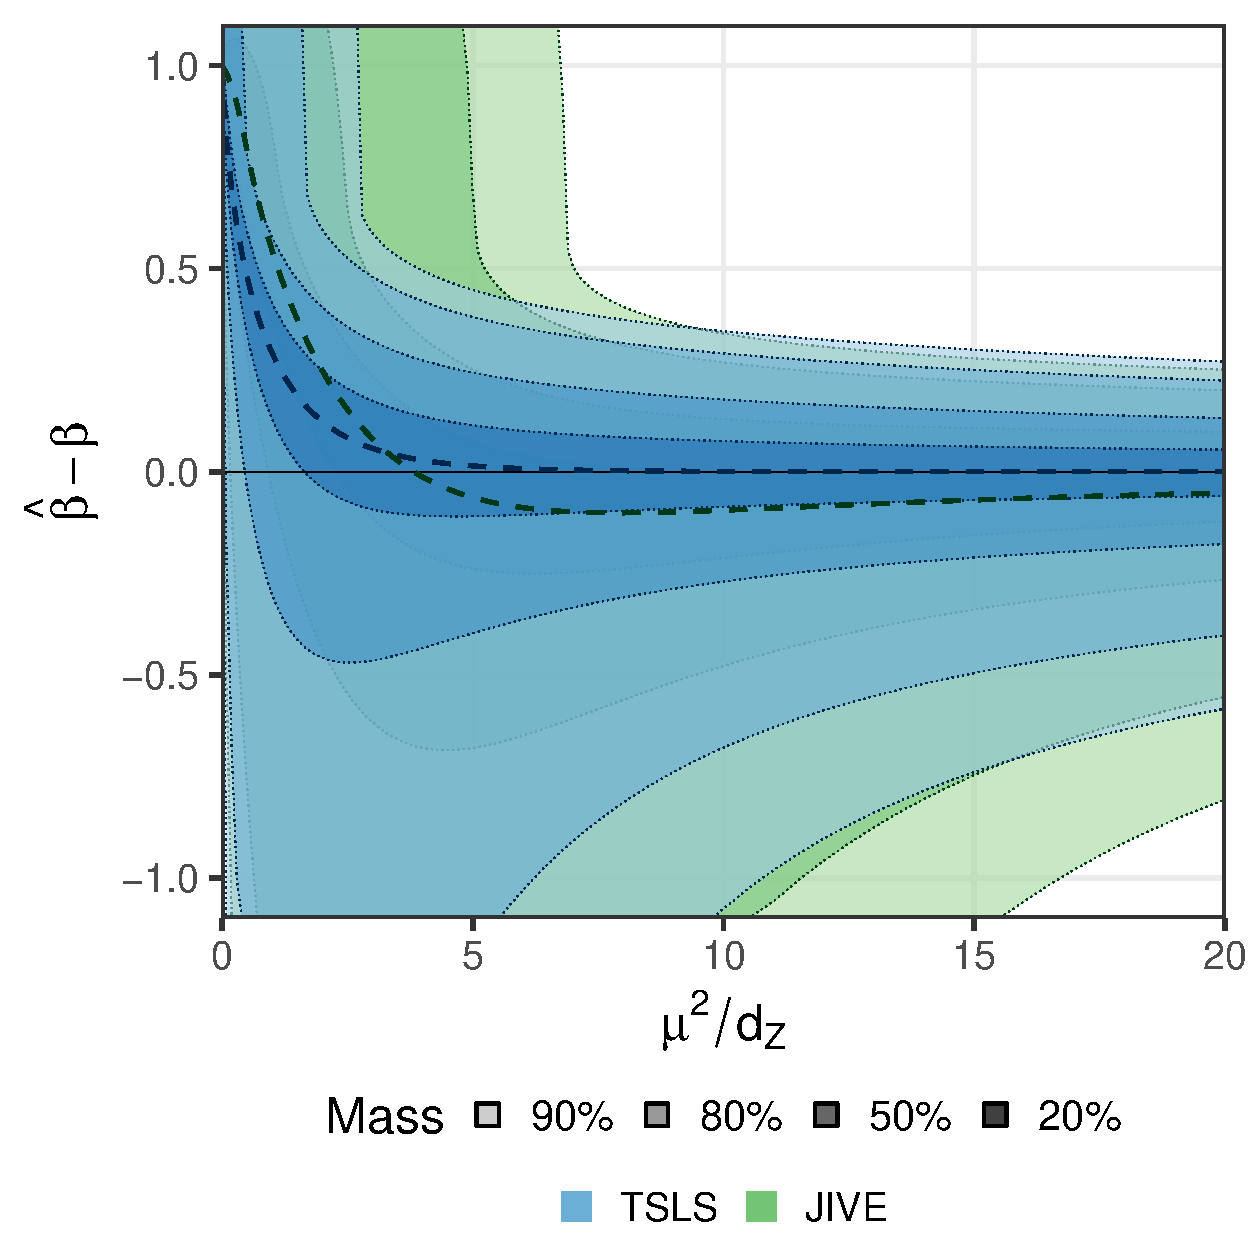
\includegraphics[width=0.4\textwidth]{figs/limit_compare_tsls_jive_median_dz1.pdf}}
%     \subfloat{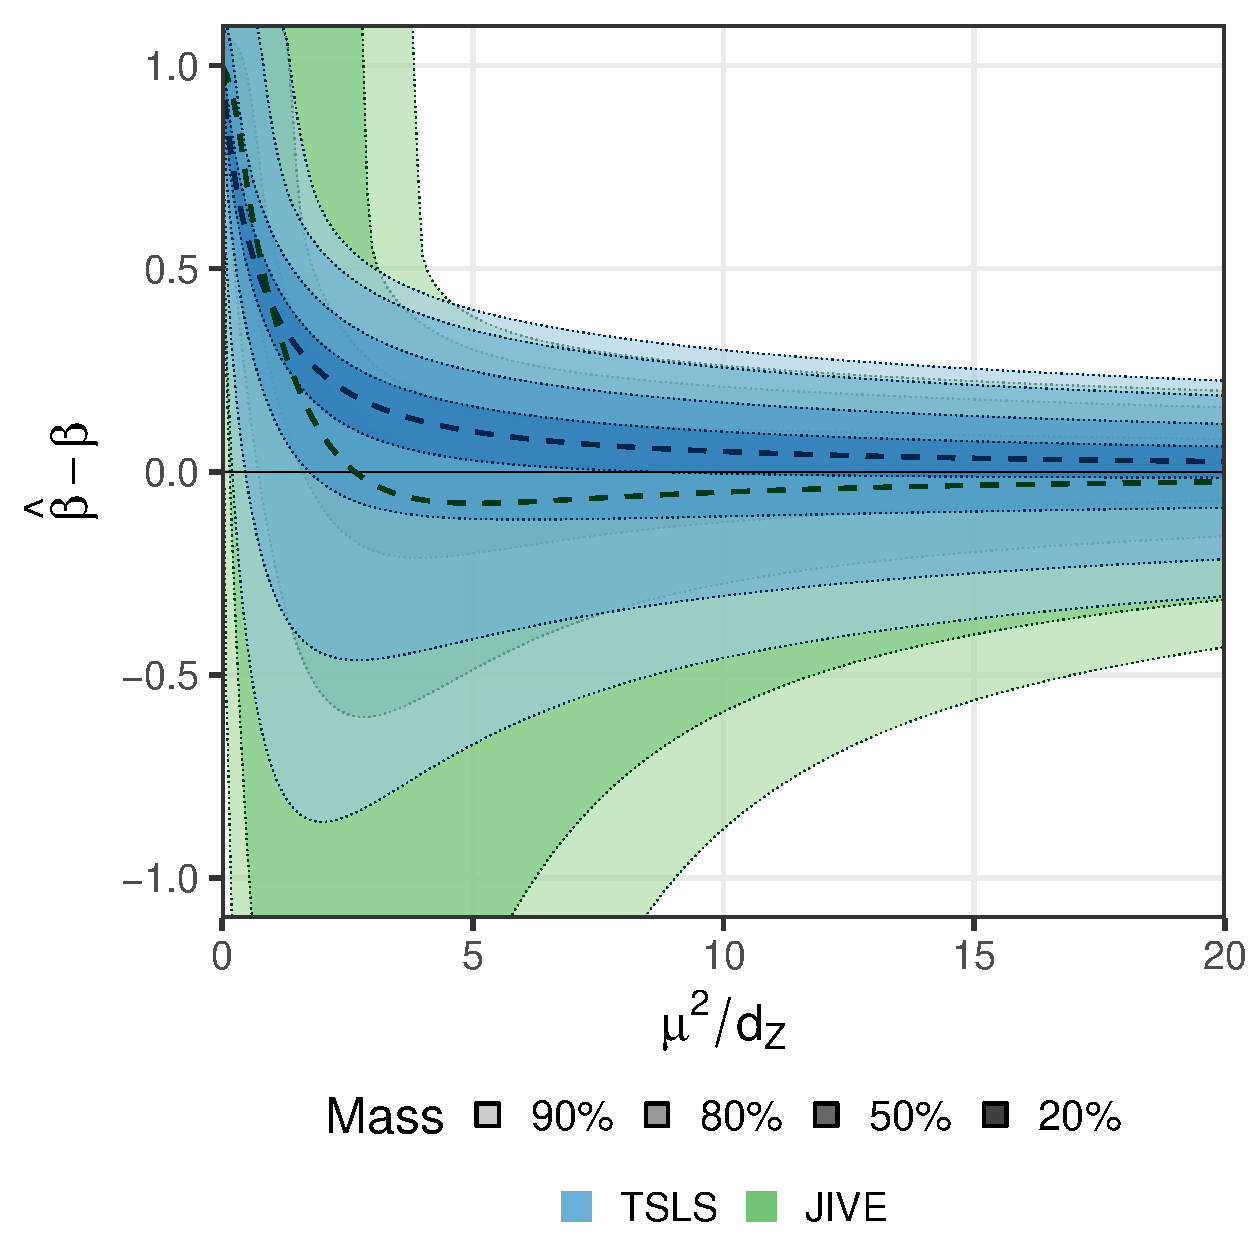
\includegraphics[width=0.4\textwidth]{figs/limit_compare_tsls_jive_median_dz2.pdf}}
%     \subfloat{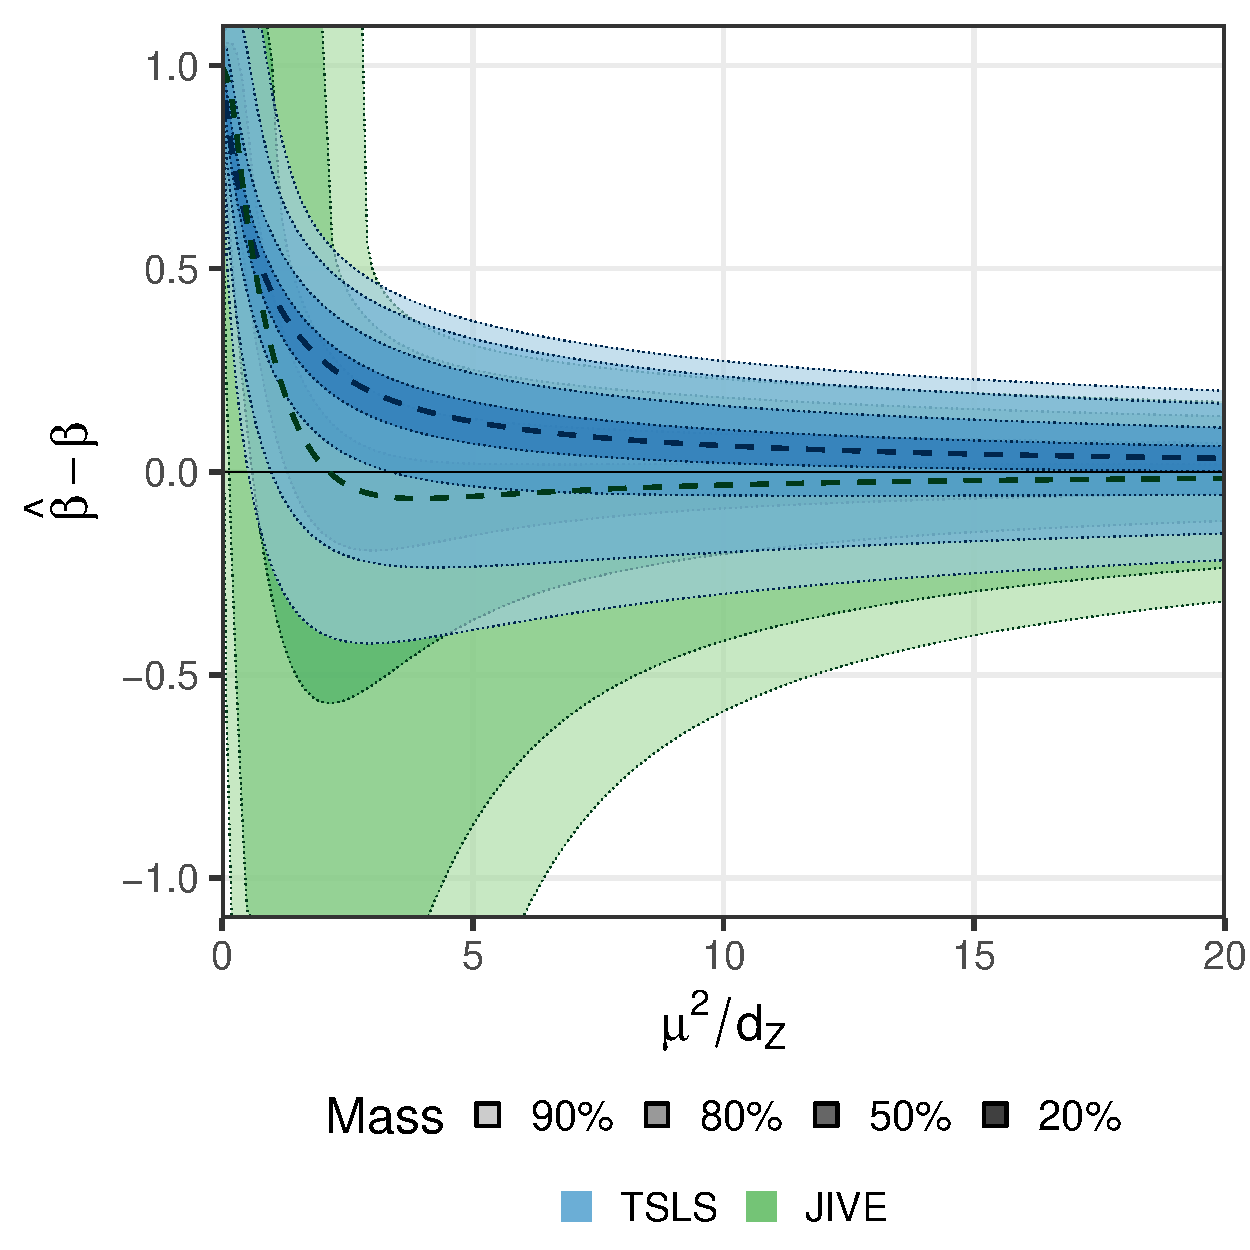
\includegraphics[width=0.4\textwidth]{figs/limit_compare_tsls_jive_median_dz3.pdf}}
%     \subfloat{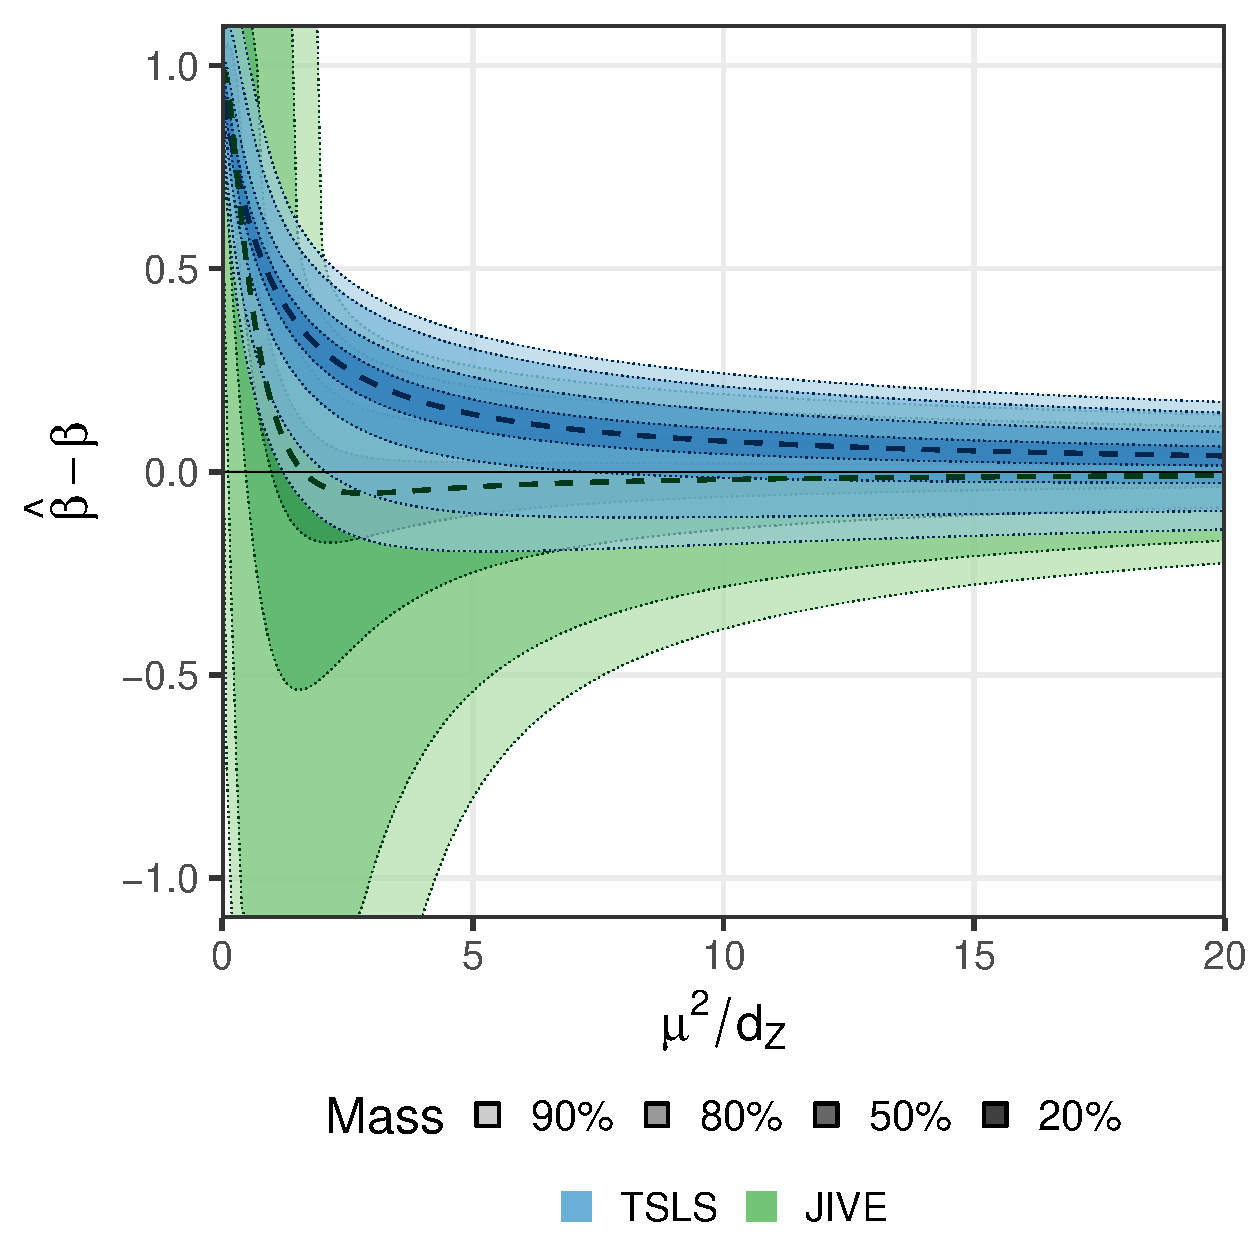
\includegraphics[width=0.4\textwidth]{figs/limit_compare_tsls_jive_median_dz5.pdf}}
%     \subfloat{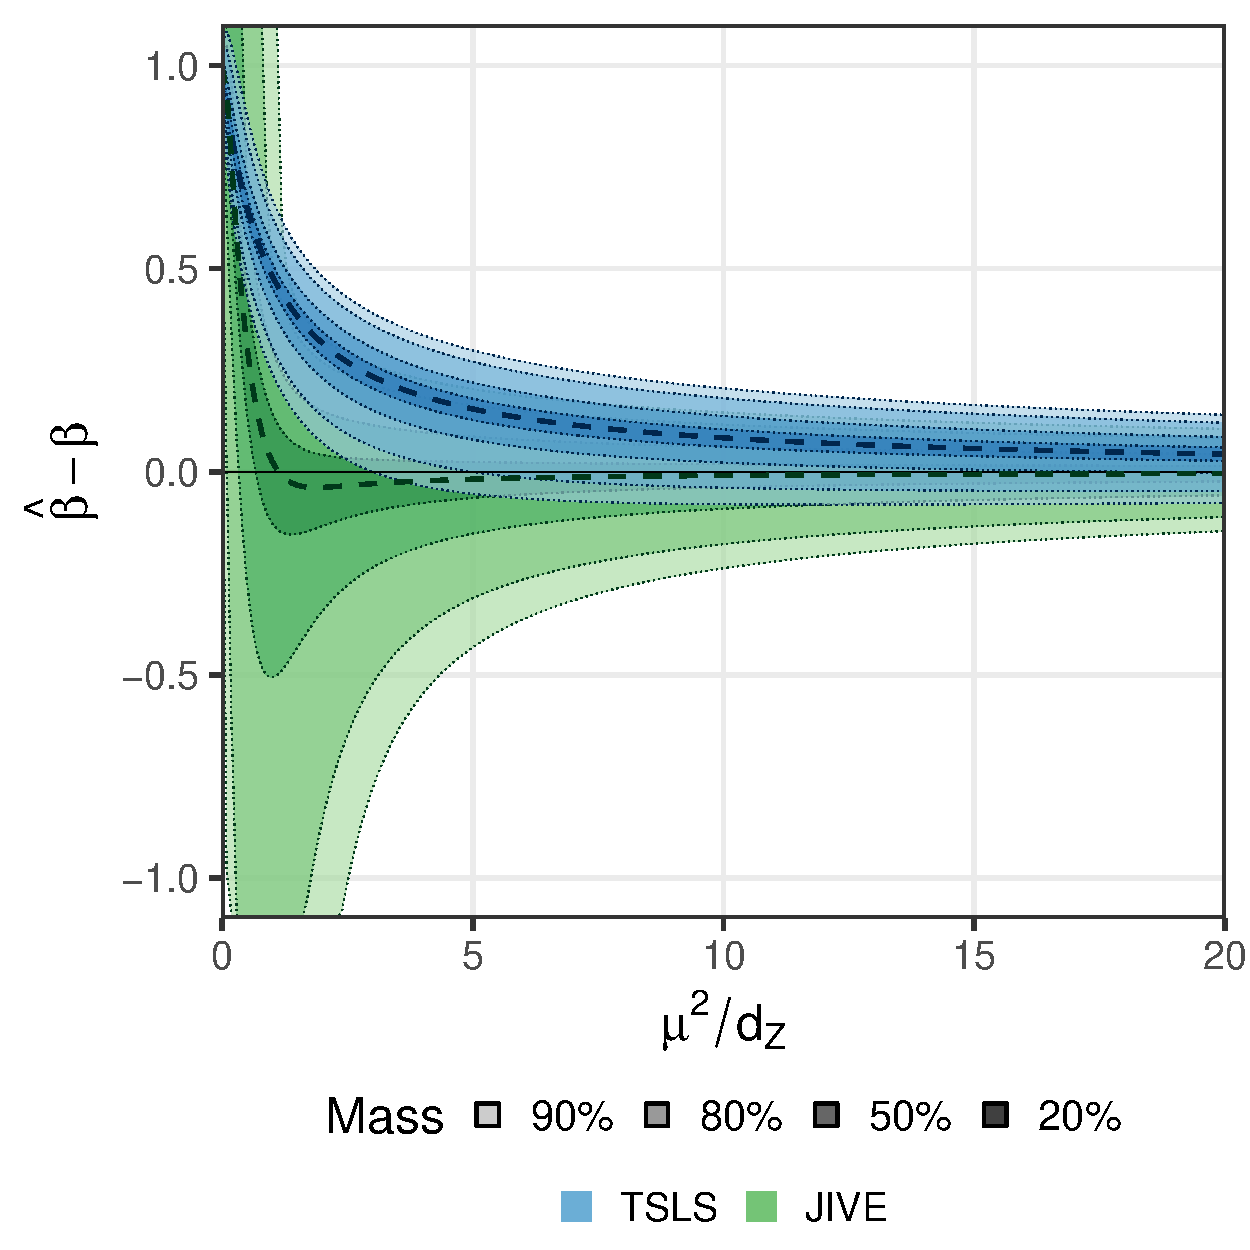
\includegraphics[width=0.4\textwidth]{figs/limit_compare_tsls_jive_median_dz10.pdf}}
%     \subfloat{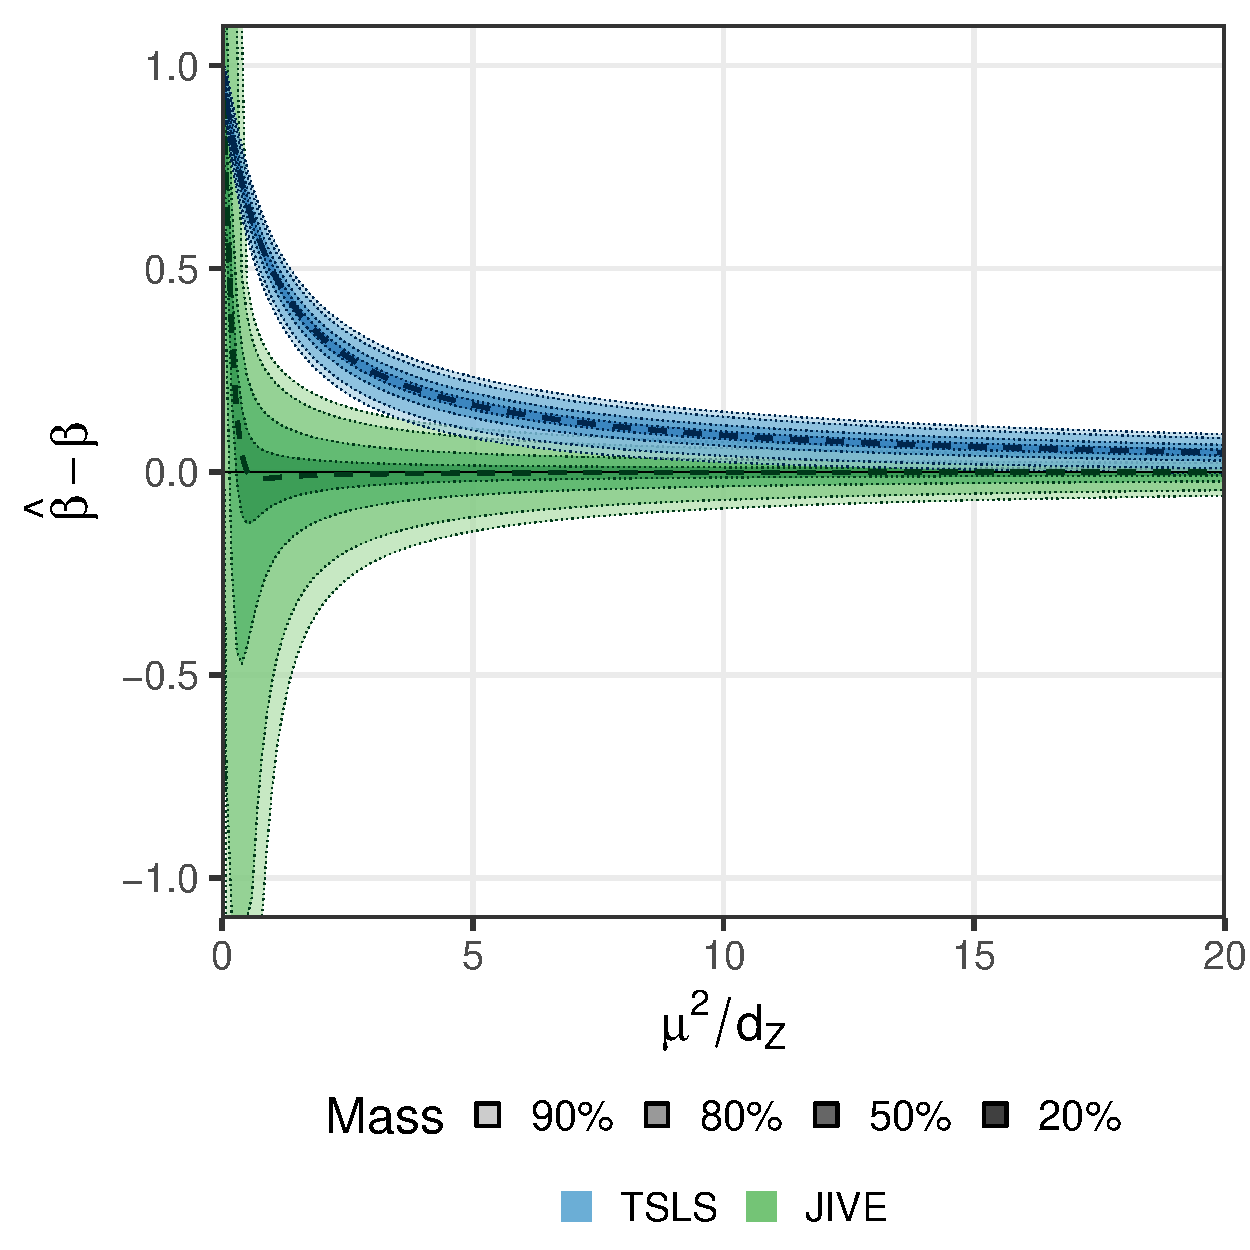
\includegraphics[width=0.4\textwidth]{figs/limit_compare_tsls_jive_median_dz50.pdf}}
    


%        \caption{\textbf{Limiting Distribution of the TSLS and JIVE Estimators.} The figure shows quantiles of the limiting distribution of the TSLS (blue) and JIVE (green) estimators for different values of the concentration parameter \(\mu^2\) (along the x-axis), and number of instruments, \(d_Z\), relative to \(\omega\), fixing \(h=0.1\). 
%        Shaded areas are colored according to their share of probability mass, as indicated by the legend.
%        } 
%        \label{fig:limt-dist-tsls-jive}
% \end{figure}
